\chapter{Implementation}
In this chapter, the implementation of the previously mentioned elements as well as the patterns of the system will be discussed.
\par
The following class diagram (see \autoref{fig:CompleteClassDiagram}) illustrates the structure of the central part of the the system being developed. It does not include any classes related to either the UI, the database, or the log, but focuses on how the system models the problem domain. 

\begin{figure}[H]
    \centering
    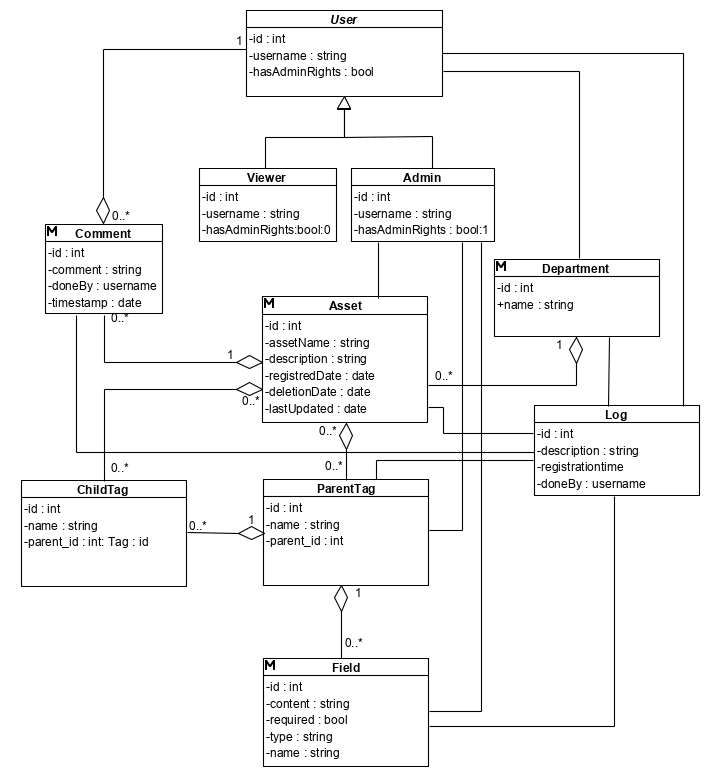
\includegraphics[width=1\textwidth]{figures/ClassDiagrams/ClassDiagramV6.PNG}
    \caption{Implementation class diagram (The bold M on some of the classes, is just a program specific thing, and can be ignored.)}
    \label{fig:CompleteClassDiagram}
\end{figure}

The class diagram in \autoref{fig:CompleteClassDiagram} shows the classes within the implemented system, as well as their internal relations. In this diagram some classes have been excluded, as these would cause unnecessary clutter in the diagram. The classes excluded from the diagram are \textit{Repositories} and \textit{ViewModels}. The excluded classes are components from the technical platform \autoref{sc:tech_intro}, as these control the data access layer and UI, and therefor do not represent key components in the logic of the system. 
\par
As seen on \autoref{fig:CompleteClassDiagram} the \textit{Log} class has an association to most of the classes within the system, as Aalborg Zoo requested that all changes should be logged. 